\chapter{group}

\begin{figure}[hbt!]
\begin{center}
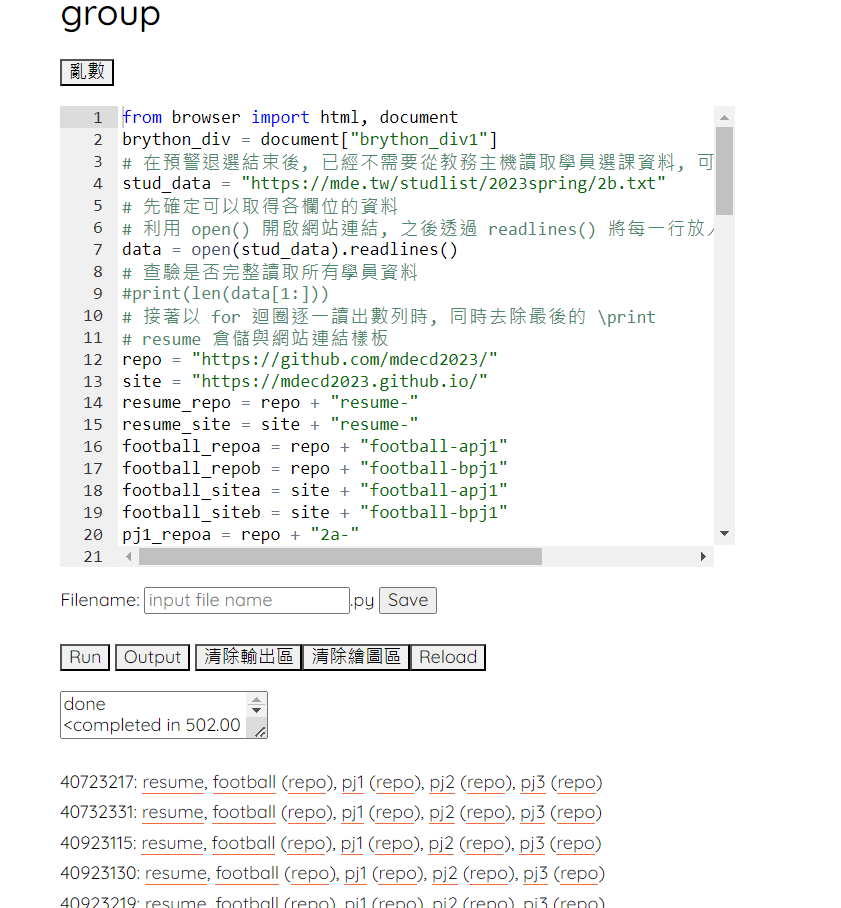
\includegraphics[width=16cm]{group}
\caption{\Large group}\label{group}
\end{center}
\end{figure}
\[
\begin{aligned}
 data = data[1:] 

random.shuffle(data) 

 

for i in data: 

    # 因為 data 第一列為資料標題, 可以利用 data[1:] 去除 

    # 而數列中每一個 element 最後的跳行符號 \n 可以利用 strip() 去除 

    stud_list = i.strip().split("\t") 

    stud_num = stud_list[0] 

    try: 

        # 若無 github 帳號則設為學號 

        github = stud_list[1] 

    except: 

        github = stud_num 

    try: 

        pj1 = stud_list[2] 

    except: 

        pj1 = "pj0" 

    try: 

        pj2 = stud_list[3] 

    except: 

        pj2 = "pj0" 

    try: 

        pj3 = stud_list[4] 

    except: 

        pj3 = "pj0" 

    #print(stud_num, github, pj1, pj2, pj3) 

    # 各學員 resume 倉儲連結 

    resume = html.A("resume", href=resume_repo+str(github)) 

    football = html.A("football", href=football_siteb) 

    football_repo = html.A("repo", href=football_repob) 

    pj1_site = html.A("pj1", href=pj1_siteb+pj1) 

    pj1_repo = html.A("repo", href=pj1_repob+pj1) 

    pj2_site = html.A("pj2", href=pj2_siteb+pj2) 

    pj2_repo = html.A("repo", href=pj2_repob+pj2) 

    pj3_site = html.A("pj3", href=pj3_siteb+pj3) 

    pj3_repo = html.A("repo", href=pj3_repob+pj3) 

    brython_div <= stud_num+": "+resume+", "+football+" ("+\ 

                   football_repo+"), "+pj1_site+" ("+pj1_repo+")"+\ 

                   ", "+pj2_site+" ("+pj2_repo+")"+\ 

                   ", "+pj3_site+" ("+pj3_repo+")" 

  

    brython_div <= html.BR() 

print("done") 

''' 

acd_tem = "https://mdecd2023.github.io/2a2-pj2ag" 

agithub = "https://github.com/mdecd2023/2a2-pj2ag" 

brython_div = document["brython_div1"] 

for i in range(1, 12): 

    url = acd_tem + str(i) 

    github = agithub + str(i) 

    brython_div <= html.A("pj2ag"+str(i), href=url) 

    brython_div <= " (" 

    brython_div <= html.A("repo", href=github) 

    brython_div <= ")" 

    bryth 
    \end{aligned}
\]\\
\newpage
